\documentclass[25pt, a0paper, portrait]{tikzposter}
\usepackage[utf8]{inputenc}
\renewcommand{\familydefault}{\sfdefault}   % sans serif font for better readibility

% % Make the default font size 36pt
% \makeatletter
% \input{biggerFont36pt.clo}
% \makeatother

\usepackage{amsmath}
\usepackage{amssymb}
\usepackage{blindtext}
\usepackage{comment}
\usetikzlibrary{arrows, shapes, trees, calc}
\usepackage{multirow}
\usepackage{multicol}

\usetheme{Default}
\usebackgroundstyle{Empty}
\usetitlestyle{Empty}
\useblockstyle[roundedcorners=6, linewidth=10pt]{Default} % Can use this line to change the stile of blocks for entire document

% Define macros to make certain things easier
\newcommand{\mtx}[1]{\begin{bmatrix} #1 \end{bmatrix}}

% Packages for drawings/diagrams
\usepackage{pgfplots}
\pgfplotsset{compat=1.15}
\usepgfplotslibrary{polar}
\usepgfplotslibrary{patchplots}

% Custom color definitions
\definecolor{Mblue}{HTML}{00274c}
\definecolor{Mmaize}{HTML}{ffcb05}
\definecolor{lightyellow}{RGB}{255,236,132}
\definecolor{lightgreen}{RGB}{161,239,10}
\definecolor{darkgreen}{RGB}{61,124,68}
\definecolor{lightblue}{RGB}{72,131,219}
\definecolor{darkblue}{RGB}{39,63,186}
\definecolor{plgreen}{RGB}{27,158,119}
\definecolor{plorange}{RGB}{217,95,2}
\definecolor{plpurple}{RGB}{117,112,179}
\definecolor{plpink}{RGB}{231,41,138}
\definecolor{lightgrey}{rgb}{0.85, 0.85, 0.85}
\definecolor{lightlightgrey}{rgb}{0.95, 0.95, 0.95}

% set the color of the block titles
\colorlet{blocktitlebgcolor}{Mblue}
\colorlet{innerblocktitlebgcolor}{Mmaize}

% Set the title info

% % \title{\parbox{0.65\linewidth}{\centering \textbf{Position Control of Parallel Combinations of Soft Actuators}}}
% \title{\LARGE{Position Control of Parallel Combinations of Soft Actuators}}
% \author{\Large{Daniel Bruder, Audrey Sedal, Ram Vasudevan, C. David Remy}}
% \institute{\large{University of Michigan}}

% \title{\parbox{0.65\linewidth}{\centering \textbf{Position Control of Parallel Combinations of Soft Actuators}}}
\title{Model-Based Control of Parallel Combinations of Soft Actuators}
\author{Daniel Bruder, Audrey Sedal, Ram Vasudevan, C. David Remy}
\institute{University of Michigan}




% BEGINNING OF DOCUMENT-------------------------------------------------------------------------------------
\begin{document}



\maketitle

% Put logos in the the top corners
\node[anchor=west] at (TP@title.west) {
\includegraphics[width=0.125\linewidth]{images/UMlogo.eps}};
\node[anchor=east] at (TP@title.east) (ROAHM) {
\includegraphics[width=0.125\linewidth]{images/ROAHMLABicon.pdf}};
\node[anchor=south] at (ROAHM.north) (RAM) {
\includegraphics[width=0.125\linewidth]{images/RAMlogo.pdf}};
\node[anchor=north] at (ROAHM.south) (CSDL) {
\includegraphics[width=0.125\linewidth]{images/csdl_logo.pdf}};

% Block 1 - Motivation
\block{Motivation: Soft robots offer potential advantages, but are difficult to control}{
    \begin{minipage}[t]{0.45\linewidth}
        Soft articulated structures in nature demonstrate benefits such as:
        \begin{multicols}{2}
        \begin{itemize}
            \setlength{\itemindent}{1in}
            \item Agility
            \item Adaptability
            \item Collision resistance
            \item Inherent safety
        \end{itemize}
        \end{multicols}
        Such characteristics are also desirable in engineered systems, but their many DOFs, nonlinear behavior, and unconventional structure make them difficult to control.
        \vspace{12pt}
        
        \begin{centering}
        \coloredbox[width=\linewidth, bgcolor=lightgrey, framecolor=red]{
        \Large{\textbf{Our goal is to derive a model of parallel combinations of soft actuators to inform the design and control of soft robots.}}
        % OUR GOAL IS TO DERIVE A MODEL OF PARALLEL COMBINATIONS OF SOFT ACTUATORS TO INFORM THE DESIGN AND CONTROL OF SOFT ROBOTS.
        }
        \end{centering}
 
        % The fiber-reinforced elastomeric enclosure (FREE) is a soft actuator composed of a fluid-filled elastomeric tube wound with reinforcing fibers (right). These fiber-reinforcements constrict the enclosed volume of the tube so that when it expands it twists and changes length a predetermined way. This customizability makes FREEs...

    \end{minipage} %
    \hspace{25pt}
    \begin{minipage}[t]{0.15\linewidth}
        \centering
        \begin{tikzfigure}
            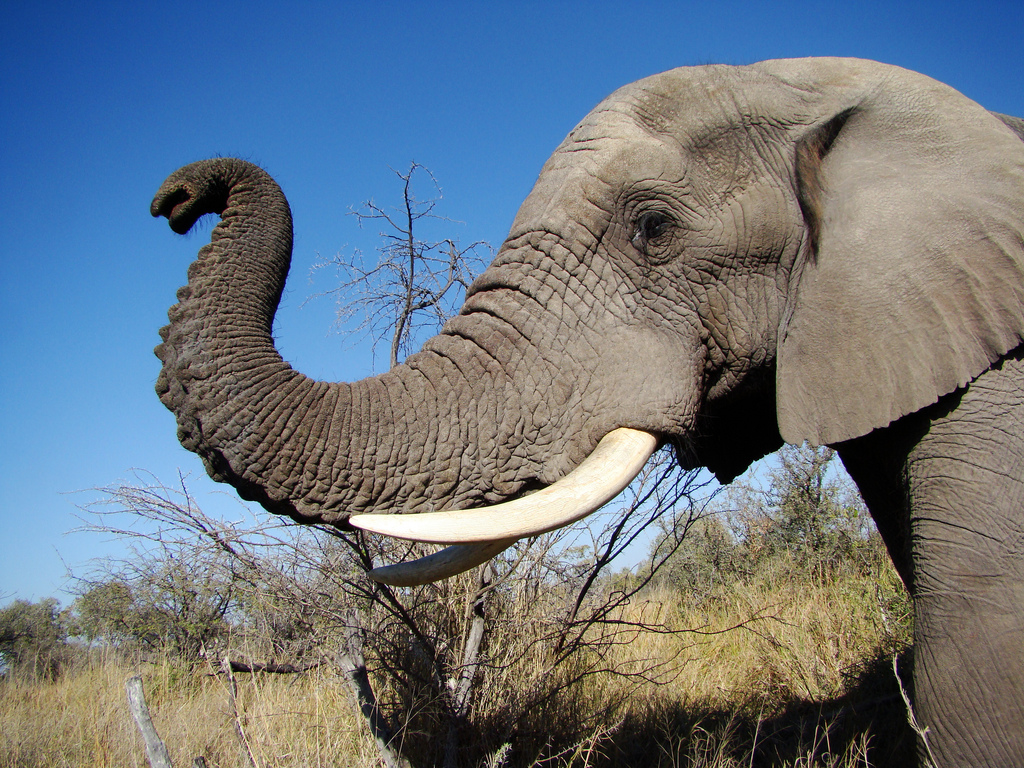
\includegraphics[width=\linewidth, height=0.075\textheight]{images/elephant.jpg}
        \end{tikzfigure}
    \end{minipage} %
    \begin{minipage}[t]{0.15\linewidth}
        \centering
        \begin{tikzfigure}
            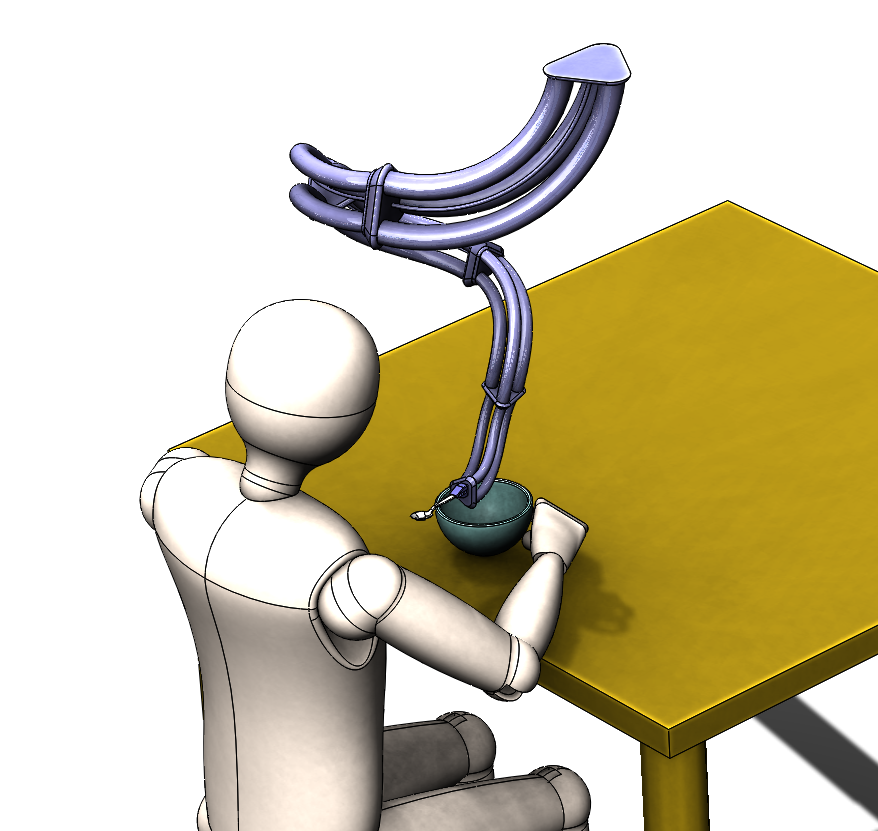
\includegraphics[width=\linewidth, height=0.075\textheight]{images/Application2.png}
        \end{tikzfigure}
    \end{minipage} %
    \begin{minipage}[t]{0.2\linewidth}
        \centering
        \begin{tikzfigure}
            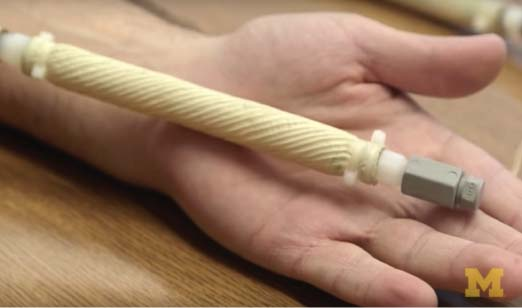
\includegraphics[width=\linewidth, height=0.075\textheight]{images/FREEhand.jpg}
        \end{tikzfigure}
    \end{minipage}
}

\begin{columns}
\column{0.5}

% Block 2 - Modeling
\colorlet{blockbodybgcolor}{lightlightgrey}
\block{Model: Actuator force depends on geometry}{
    \innerblock[roundedcorners=4]{Individual Actuators}{
    \begin{minipage}[c]{\linewidth}
        The fiber-reinforced elastomeric enclosure (FREE) is a soft actuator composed of a fluid-filled elastomeric tube wound with reinforcing fibers. A pressurized FREE generates a force ($F$) and moment ($M$) about its central axis due to the fiber tensile force ($T$) pulling at an angle ($\Gamma$). 
        This force and moment constitute the generalized force vector $\vec{\tau}$:
        \begin{equation*}
            \vec{\tau} = \mtx{F, & M}^T
        \end{equation*}
        % Given a pressure, the fiber angle $\Gamma$ determines the ratio between the force and moment.
    \end{minipage}
    
    \vspace{25pt}
    
    % Force/Moment diagrams
    \begin{minipage}[c]{0.5\linewidth}
        \centering
        \begin{tikzfigure}
            \centering
            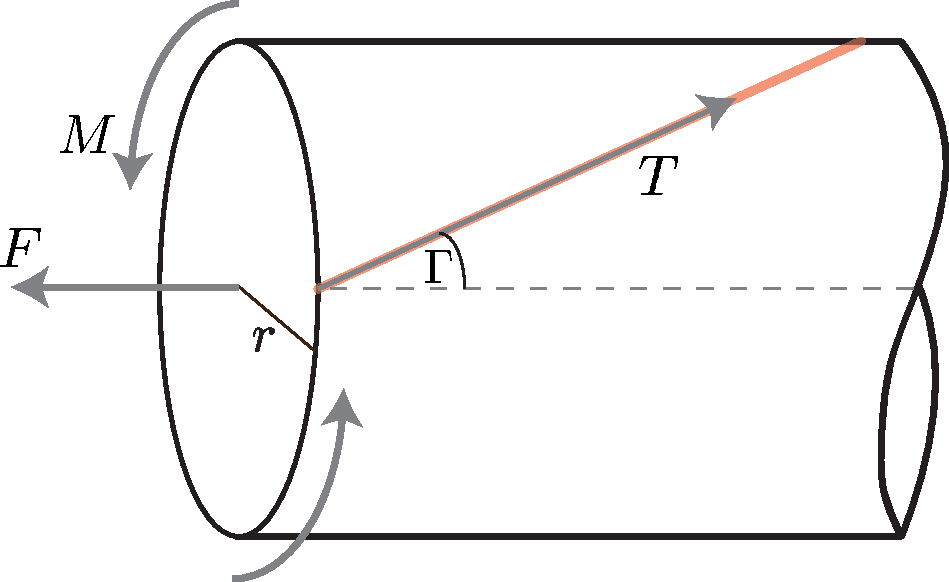
\includegraphics[width=0.8\linewidth]{images/fiberTension.pdf}
        \end{tikzfigure}
        \vspace{50pt}
    \end{minipage}
    \begin{minipage}[c]{0.5\linewidth}
        \centering
        \begin{tikzpicture}
            \begin{axis}[
                xlabel={\small{$\Gamma$}},
                ylabel={\small{$F/M$}},
                ymin=-10, ymax=10, ytick={0}, ylabel near ticks,
                xmin=0, xmax=90, xtick={0,54.7,90}, xticklabel=$\pgfmathprintnumber{\tick}^\circ$, xlabel near ticks,
                tick label style={font=\small},
                width=0.75\linewidth,
                height=3.5in,
                anchor=center,
                ]
                \addplot [domain=0:90, dashed] {0};
                \addplot [domain=1:90, samples=100] {(1-2*cot(x)^2) / (2*cot(x))};
                \addplot [mark=none, dashed] coordinates {(54.7,-10) (54.7,10)};
                \end{axis};
        \end{tikzpicture}
    \end{minipage}

    % Introduction of parameters
    \begin{minipage}[c]{0.45\linewidth}
        The \emph{relaxed} (unpressurized) geometry of a cylindrical FREE is described by its
        \begin{multicols}{2}
        \begin{itemize}
            \setlength{\itemindent}{0.5in}
            \item Radius ($R$)
            \item Length ($L$)
            % \item Fiber angle ($\Gamma$)
        \end{itemize}
        \end{multicols}
        % its radius ($R$), length ($L$), and fiber angle ($\Gamma$).
        The \emph{deformed} geometry is described by:
        \begin{itemize}
            \setlength{\itemindent}{0.5in}
            \item Length change ($\Delta l$)
            \item Twist ($\Delta \phi$)
        \end{itemize}
        % the change in length ($\Delta l$) and twist ($\Delta \phi$),
        which constitute the state vector $\vec{q}$:
        \begin{equation*}
            \vec{q} = \mtx{\Delta l, & \Delta \phi}^T
        \end{equation*}
    \end{minipage}
    \hspace{25pt}
    \begin{minipage}[c]{0.5\linewidth}
        \centering
        \begin{tikzfigure}
            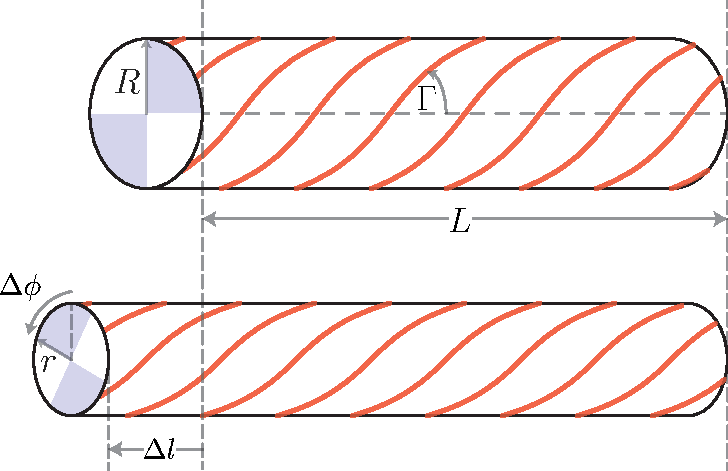
\includegraphics[width=\linewidth]{images/FREEstate_noLabels3.pdf}
        \end{tikzfigure}
    \end{minipage}
    
    \vspace{25pt}
    
    Energy conservation dictates that that the mechanical power generated by the FREE must equal the fluid power that goes into the FREE:
    
    \vspace{12pt}
    \begin{centering}
    \coloredbox[width=0.65\linewidth, framecolor=lightgrey, bgcolor=lightgrey]{
    \begin{align*}
        P_\text{mech} &= P_\text{fluid} =
        \dot{\vec{q}}^{\,T} \vec{\tau} = \dot{V}^T p 
        \hspace{25pt} \implies \hspace{25pt}
        \vec{\tau} = \bar{J}_q^T p
    \end{align*}
    }
    \end{centering}
    where $V$ is the volume, $p$ is the pressure, and $\bar{J}_q (\vec{q}) = \frac{\partial V}{\partial \vec{q}}$ is called the \emph{fluid~Jacobian}.
    }
    
    \vspace{36pt}
    \innerblock[roundedcorners=4]{Parallel Combinations of Actuators}{
    \begin{minipage}[c]{0.3\linewidth}
        \centering
        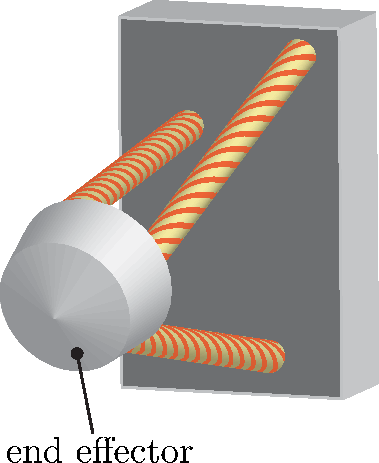
\includegraphics[width=\linewidth]{images/parallelDiagram-v2.pdf}
    \end{minipage}
    \hspace{25pt}
    \begin{minipage}[c]{0.65\linewidth}
        A parallel combination of FREEs share a common end effector.
        %Since the generalized force of an individual actuator is linear in $p$, 
        The net force generated by $n$ FREEs ($\vec{f}$) is the sum of the individual forces:
        
        \vspace{18pt}
        \begin{centering}
        \coloredbox[width=0.65\linewidth, bgcolor=lightgrey, framecolor=lightgrey]{
        \begin{equation*}
            \vec{f}(\vec{x}, \vec{p}) = \sum_{i=1}^{n} \bar{J}^T_{x,i} (\vec{x}) \, p_i
            = \bar{J}_x^T (\vec{x}) \vec{p}
        \end{equation*}
        }
        \end{centering}
        
        where $\vec{x}$ is the state of the end effector, $\vec{p} = \mtx{p_1 & \cdots & p_n}$ is a vector containing the pressure of all $n$ FREEs, and $\bar{J}_x$ is the net fluid Jacobian expressed in end effector coordinates.
    \end{minipage}
    
    \begin{minipage}[c]{0.55\linewidth}
        The \emph{force zonotope} ($\mathcal{Z}$) describes the set of forces that can be generated by a parallel combination of FREEs at a specific state, $\vec{x}$:
        
        \vspace{18pt}
        \begin{centering}
        \coloredbox[width=0.75\linewidth, framecolor=lightgrey, bgcolor=lightgrey]{
        \begin{equation*}
            \mathcal{Z}(\vec{x}) = \left\{ \bar{J}_x^T (\vec{x}) \vec{p} : p_i \in [0, p_i^\text{max}] \right\}
        \end{equation*}
        }
        \end{centering}
        
        This zonotope can be used to:
        \begin{itemize}
            \setlength{\itemindent}{1in}
            \item Determine feasible local motions
            \item Inform system design
            \item Find the limits of the workspace
        \end{itemize}
        % inform the design of systems that require control authority in certain directions, or to investigate the limits of the workspace of the 
    \end{minipage}
    \hspace{25pt}
    \begin{minipage}[c]{0.4\linewidth}
        \centering
        \begin{tikzfigure}
\centering

\def\scl{0.45} % define scale variable for plots

\begin{tikzpicture}
% Diagram and plot
\matrix [row sep=0.25cm, column sep=0cm, style={align=center}] (my matrix) at (0,0)
{

\node[anchor=center] (diagram) {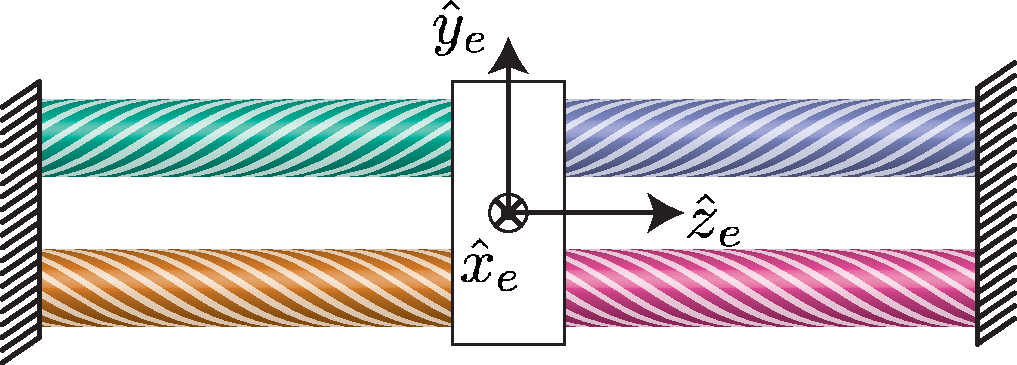
\includegraphics[width=\linewidth]{images/zntpExampleRig4.pdf}};

\\

\begin{axis}[
    view={90}{0},
    axis lines=center,
    % axis equal image,
    xlabel={$M^{\hat{x}_e}$},
    ylabel={$F^{\hat{z}_e}$},
    zlabel={$M^{\hat{z}_e}$},
    ymin=-7, ymax=7, ytick={0}, %ylabel near ticks,
    xmin=-5, xmax=10, xtick={0}, %xticklabel=$\pgfmathprintnumber{\tick}^\circ$, xlabel near ticks, 
    zmin=-7, zmax=7, ztick={0}, %z dir=reverse,
    xlabel style={anchor=north}, ylabel style={anchor=north},
    % scale=\scl,
    anchor=center,
    name=plot4,
    width=\linewidth,
    height=5.25in,
    line width=5pt,
    ]
    \def\pa{(-2,-3,2)}
    \def\pb{(2,-3,-2)}
    \def\pc{(2,3,-2)}
    \def\pd{(-2,3,2)}

    % connector lines for perspective
    \addplot3[dotted, line width=2pt] coordinates {(0,0,0) (-2,-3,0)};
    \addplot3[dotted, line width=2pt] coordinates {(-2,-3,0) \pa}; 
    \addplot3[dotted, line width=2pt] coordinates {(0,0,0) (2,-3,0)};
    \addplot3[dotted, line width=2pt] coordinates {(2,-3,0) \pb};
    \addplot3[dotted, line width=2pt] coordinates {(0,0,0) (2,3,0)};
    \addplot3[dotted, line width=2pt] coordinates {(2,3,0) \pc};
    \addplot3[dotted, line width=2pt] coordinates {(0,0,0) (-2,3,0)};
    \addplot3[dotted, line width=2pt] coordinates {(-2,3,0) \pd};
    % faces of shape
    \addplot3[patch, opacity=0.3, fill=black!20, faceted color=black, patch type=rectangle, line width=1pt] 
        coordinates {
                    (0,0,0) \pa (0,-6,0) \pb
                    (0,0,0) \pb (4,0,-4) \pc
                    (0,0,0) \pc (0,6,0) \pd
                    (0,0,0) \pd (-4,0,4) \pa
                    };
    
    % force vectors for each FREE                
    \addplot3[->, line width=5pt, plgreen] coordinates {(0,0,0) \pa};
    \addplot3[->, line width=5pt, plorange] coordinates {(0,0,0) \pb};
    \addplot3[->, line width=5pt, plpurple] coordinates {(0,0,0) \pc};
    \addplot3[->, line width=5pt, plpink] coordinates {(0,0,0) \pd};
\end{axis};

\\
};

\end{tikzpicture}
    
\end{tikzfigure}
    \end{minipage}
    }
}

\column{0.5}

% Block 3 - Experiment
\colorlet{blockbodybgcolor}{white}
\block{Validation: Model predicts forces generated by FREEs}{
    We measured the force and moment generated by a parallel combination of three FREEs at various pressure combinations and compared them to the forces predicted by the model.
    \begin{minipage}[c]{0.65\linewidth}
        \centering
        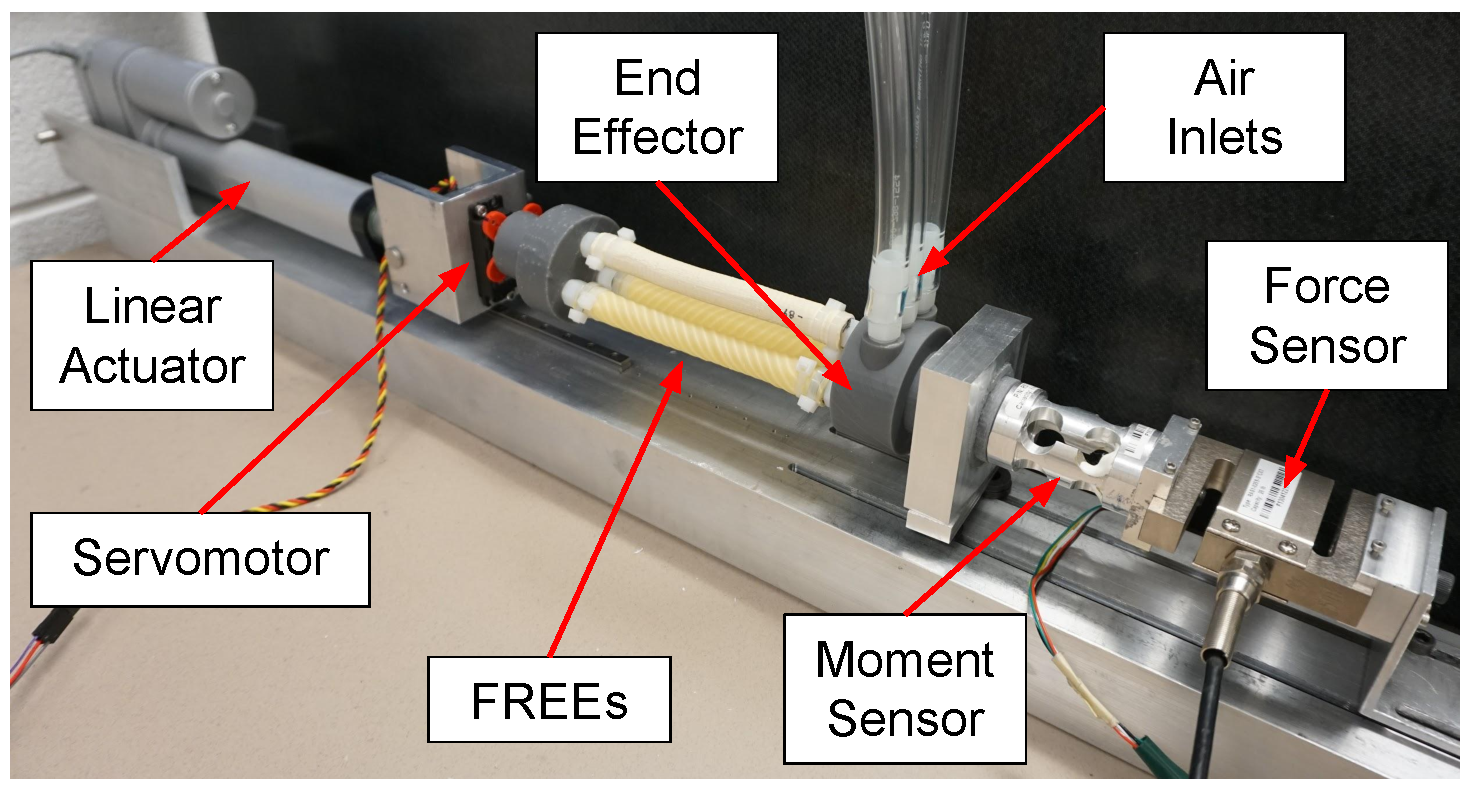
\includegraphics[width=\linewidth]{images/rig_labeled.pdf}
    \end{minipage}
    \hspace{10pt}
    \begin{minipage}[c]{0.3\linewidth}
        \centering
        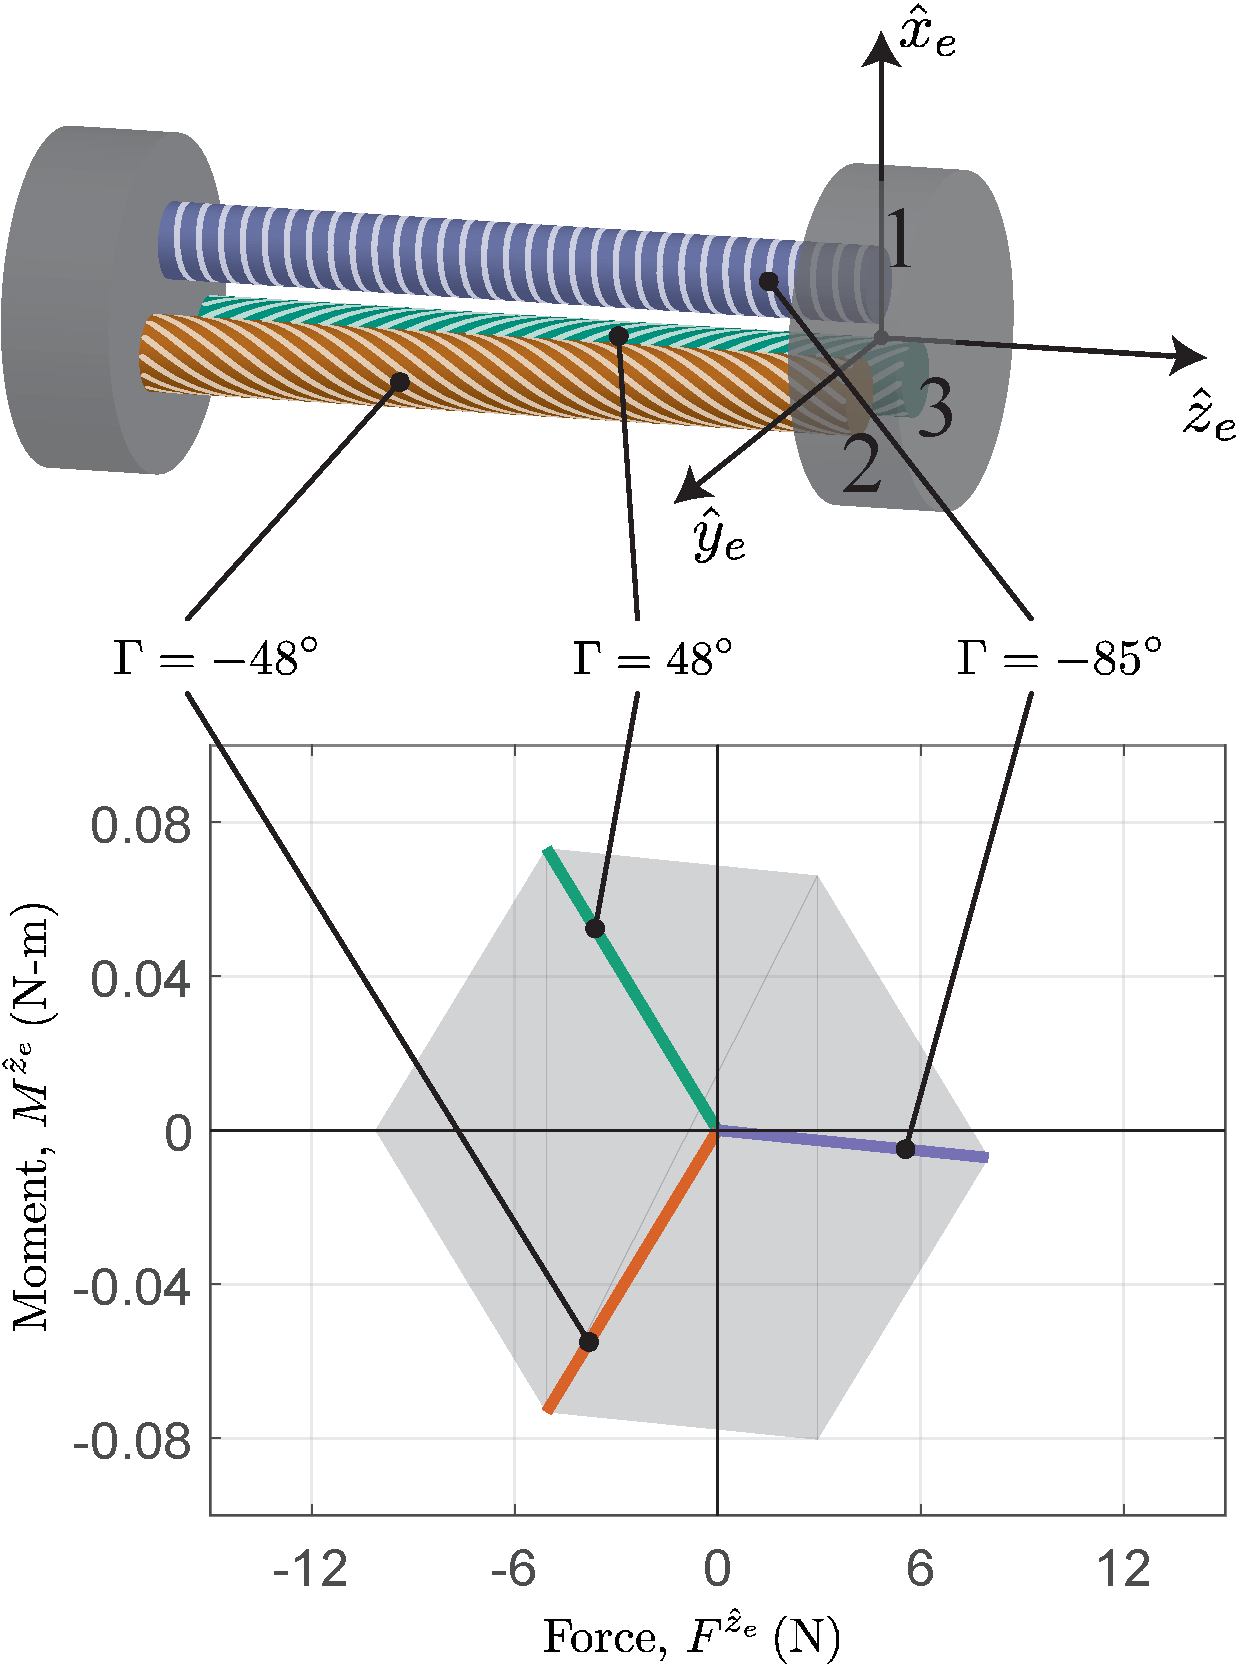
\includegraphics[width=\linewidth]{images/rigDiagram_wlabels10.pdf}
    \end{minipage}
    \\
    \begin{minipage}[c]{\linewidth}
        \centering
        \def\picScale{0.08}    % define variable for scaling all pictures evenly
\def\plotScale{0.2}    % define variable for scaling all plots evenly
\def\colWidth{0.22\linewidth}

\begin{tikzpicture}
\tikzstyle{every node}=[font=\small]    % change font size

% \draw[help lines] (0,0) grid (4,2);
\matrix [row sep=0cm, column sep=0cm, style={align=center}] (my matrix) at (current bounding box.center) %(0,0)
{
& \node (q1) {(a) $\Delta l = 0, \Delta \phi = 0$}; & \node (q2) {(b) $\Delta l = 5\text{mm}, \Delta \phi = 0$}; & \node (q3) {(c) $\Delta l = 0, \Delta \phi = 20^\circ$}; & \node (q4) {(d) $\Delta l = 5\text{mm}, \Delta \phi = 20^\circ$};

\\

&
\node[style={anchor=center}] {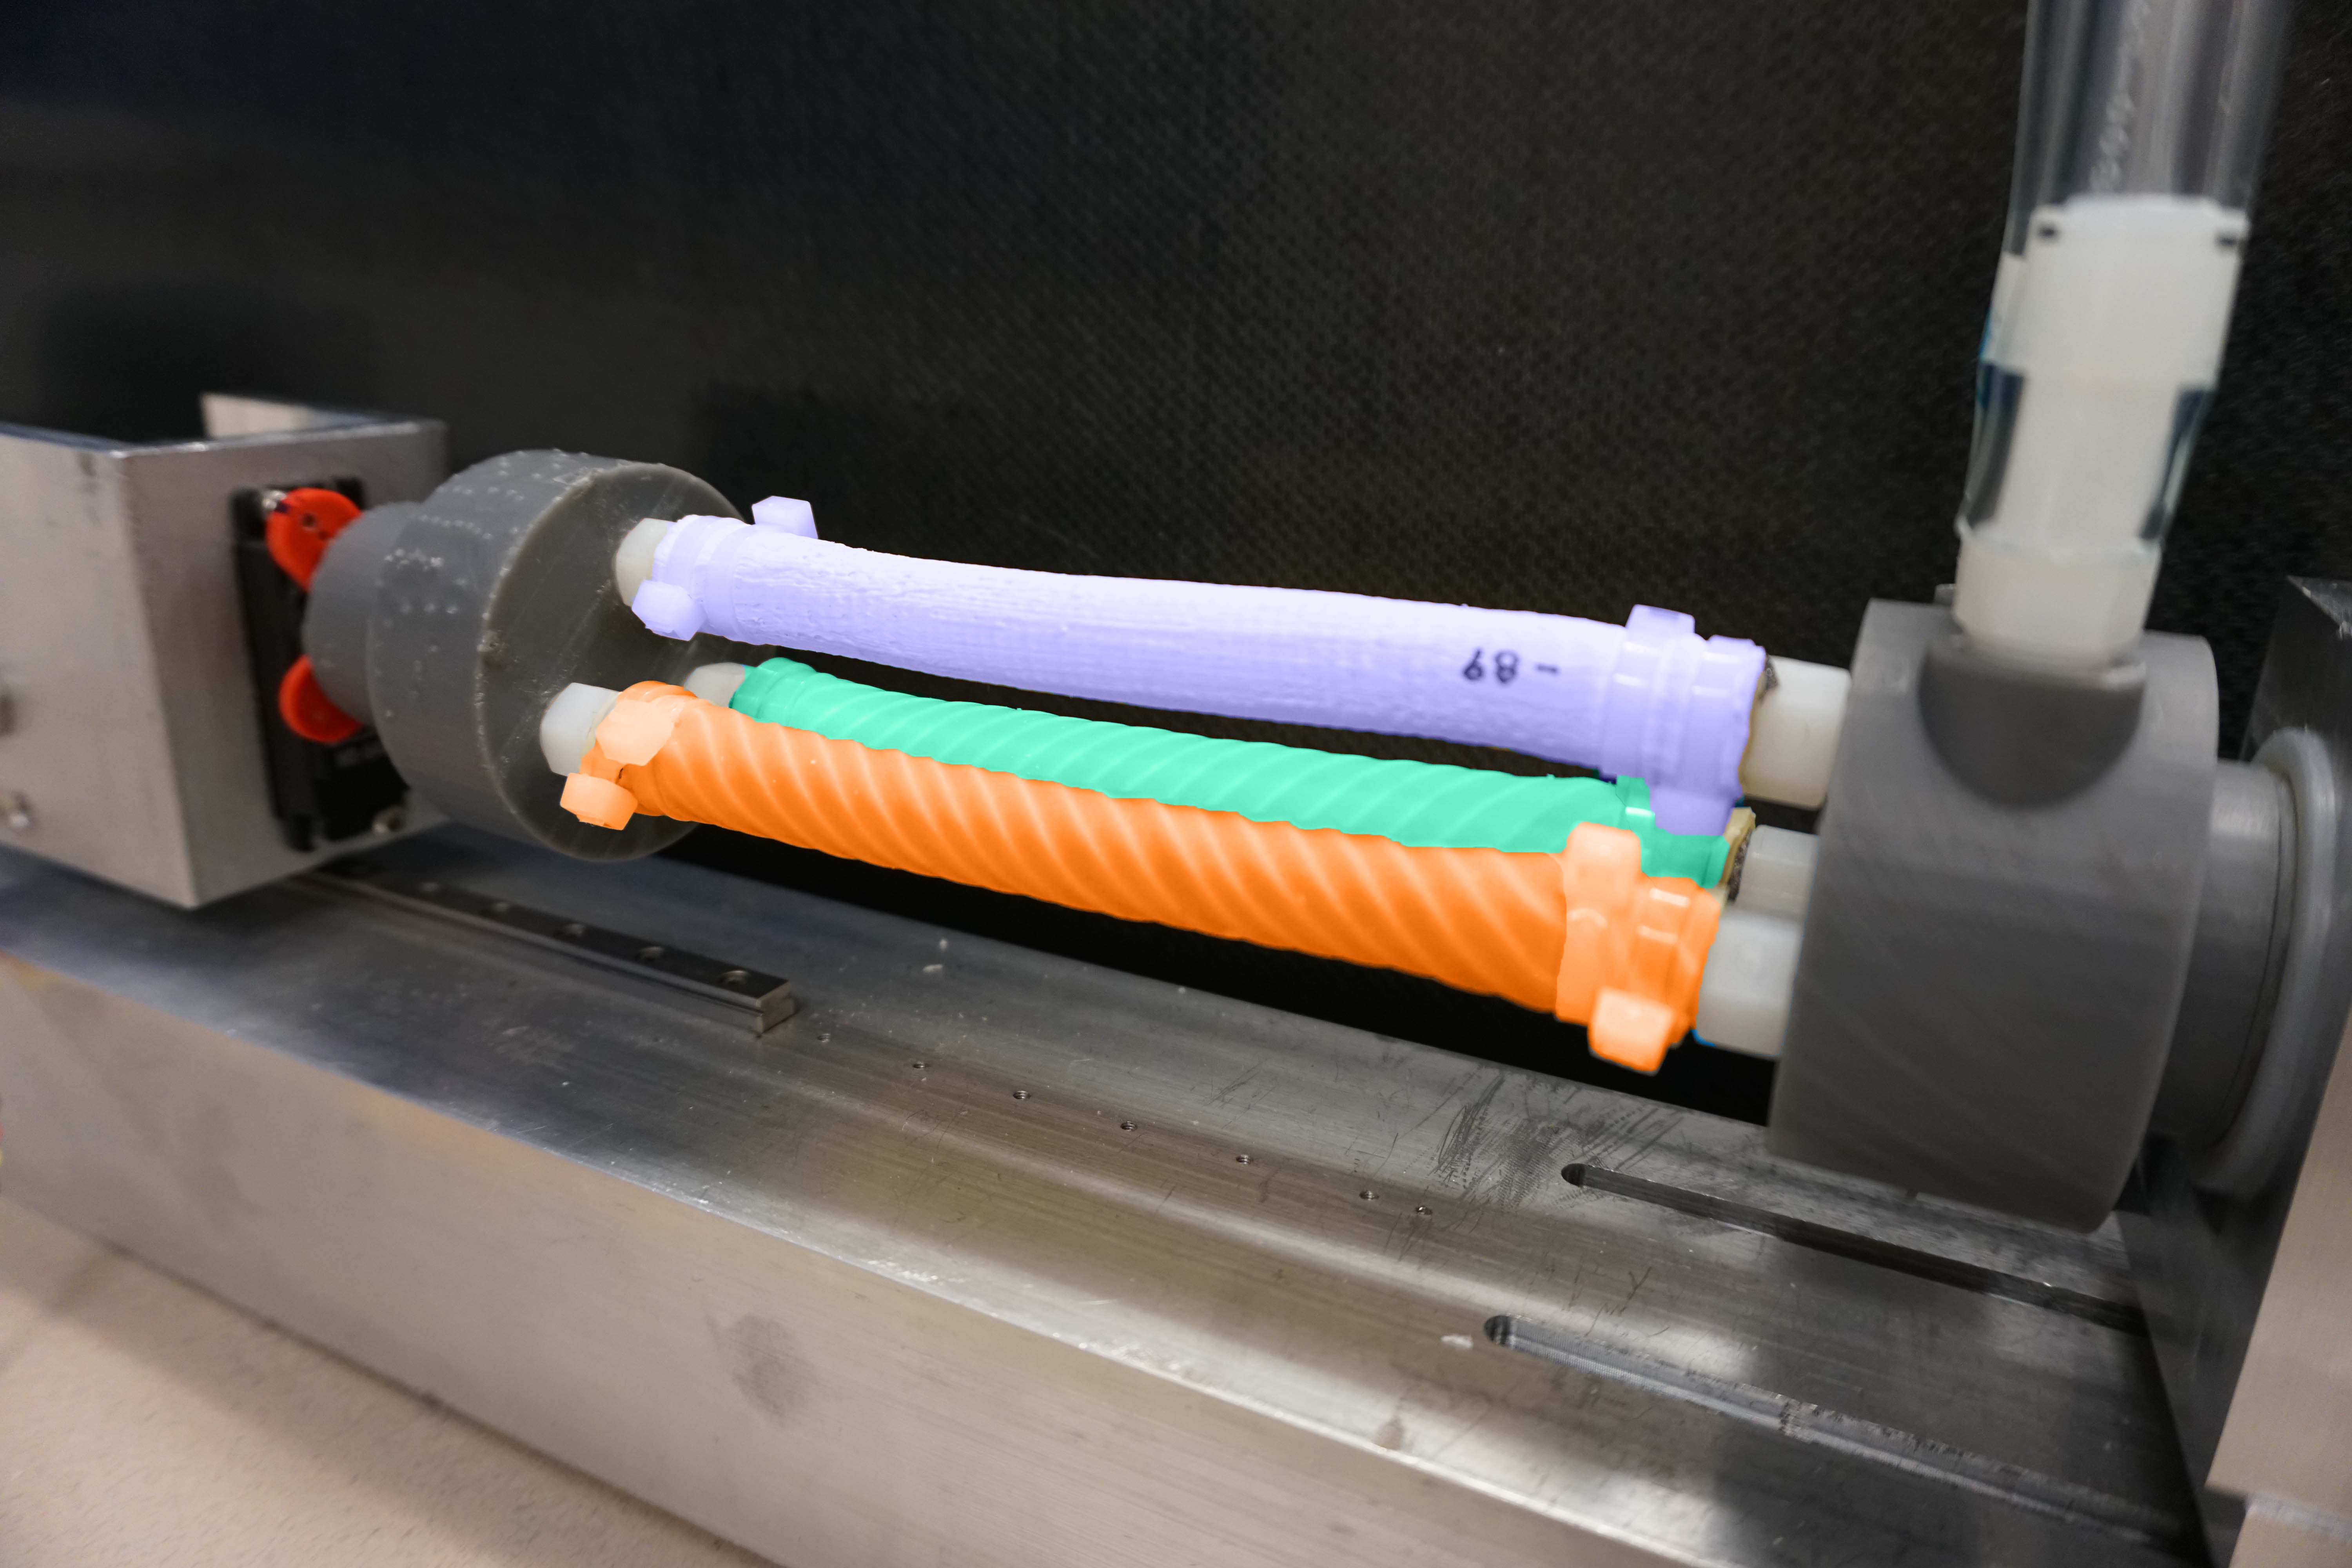
\includegraphics[width=\colWidth]{images/photos/s0w0pic_colored.jpg}}; %\fill[blue] (0,0) circle (2pt);
&
\node[style={anchor=center}] {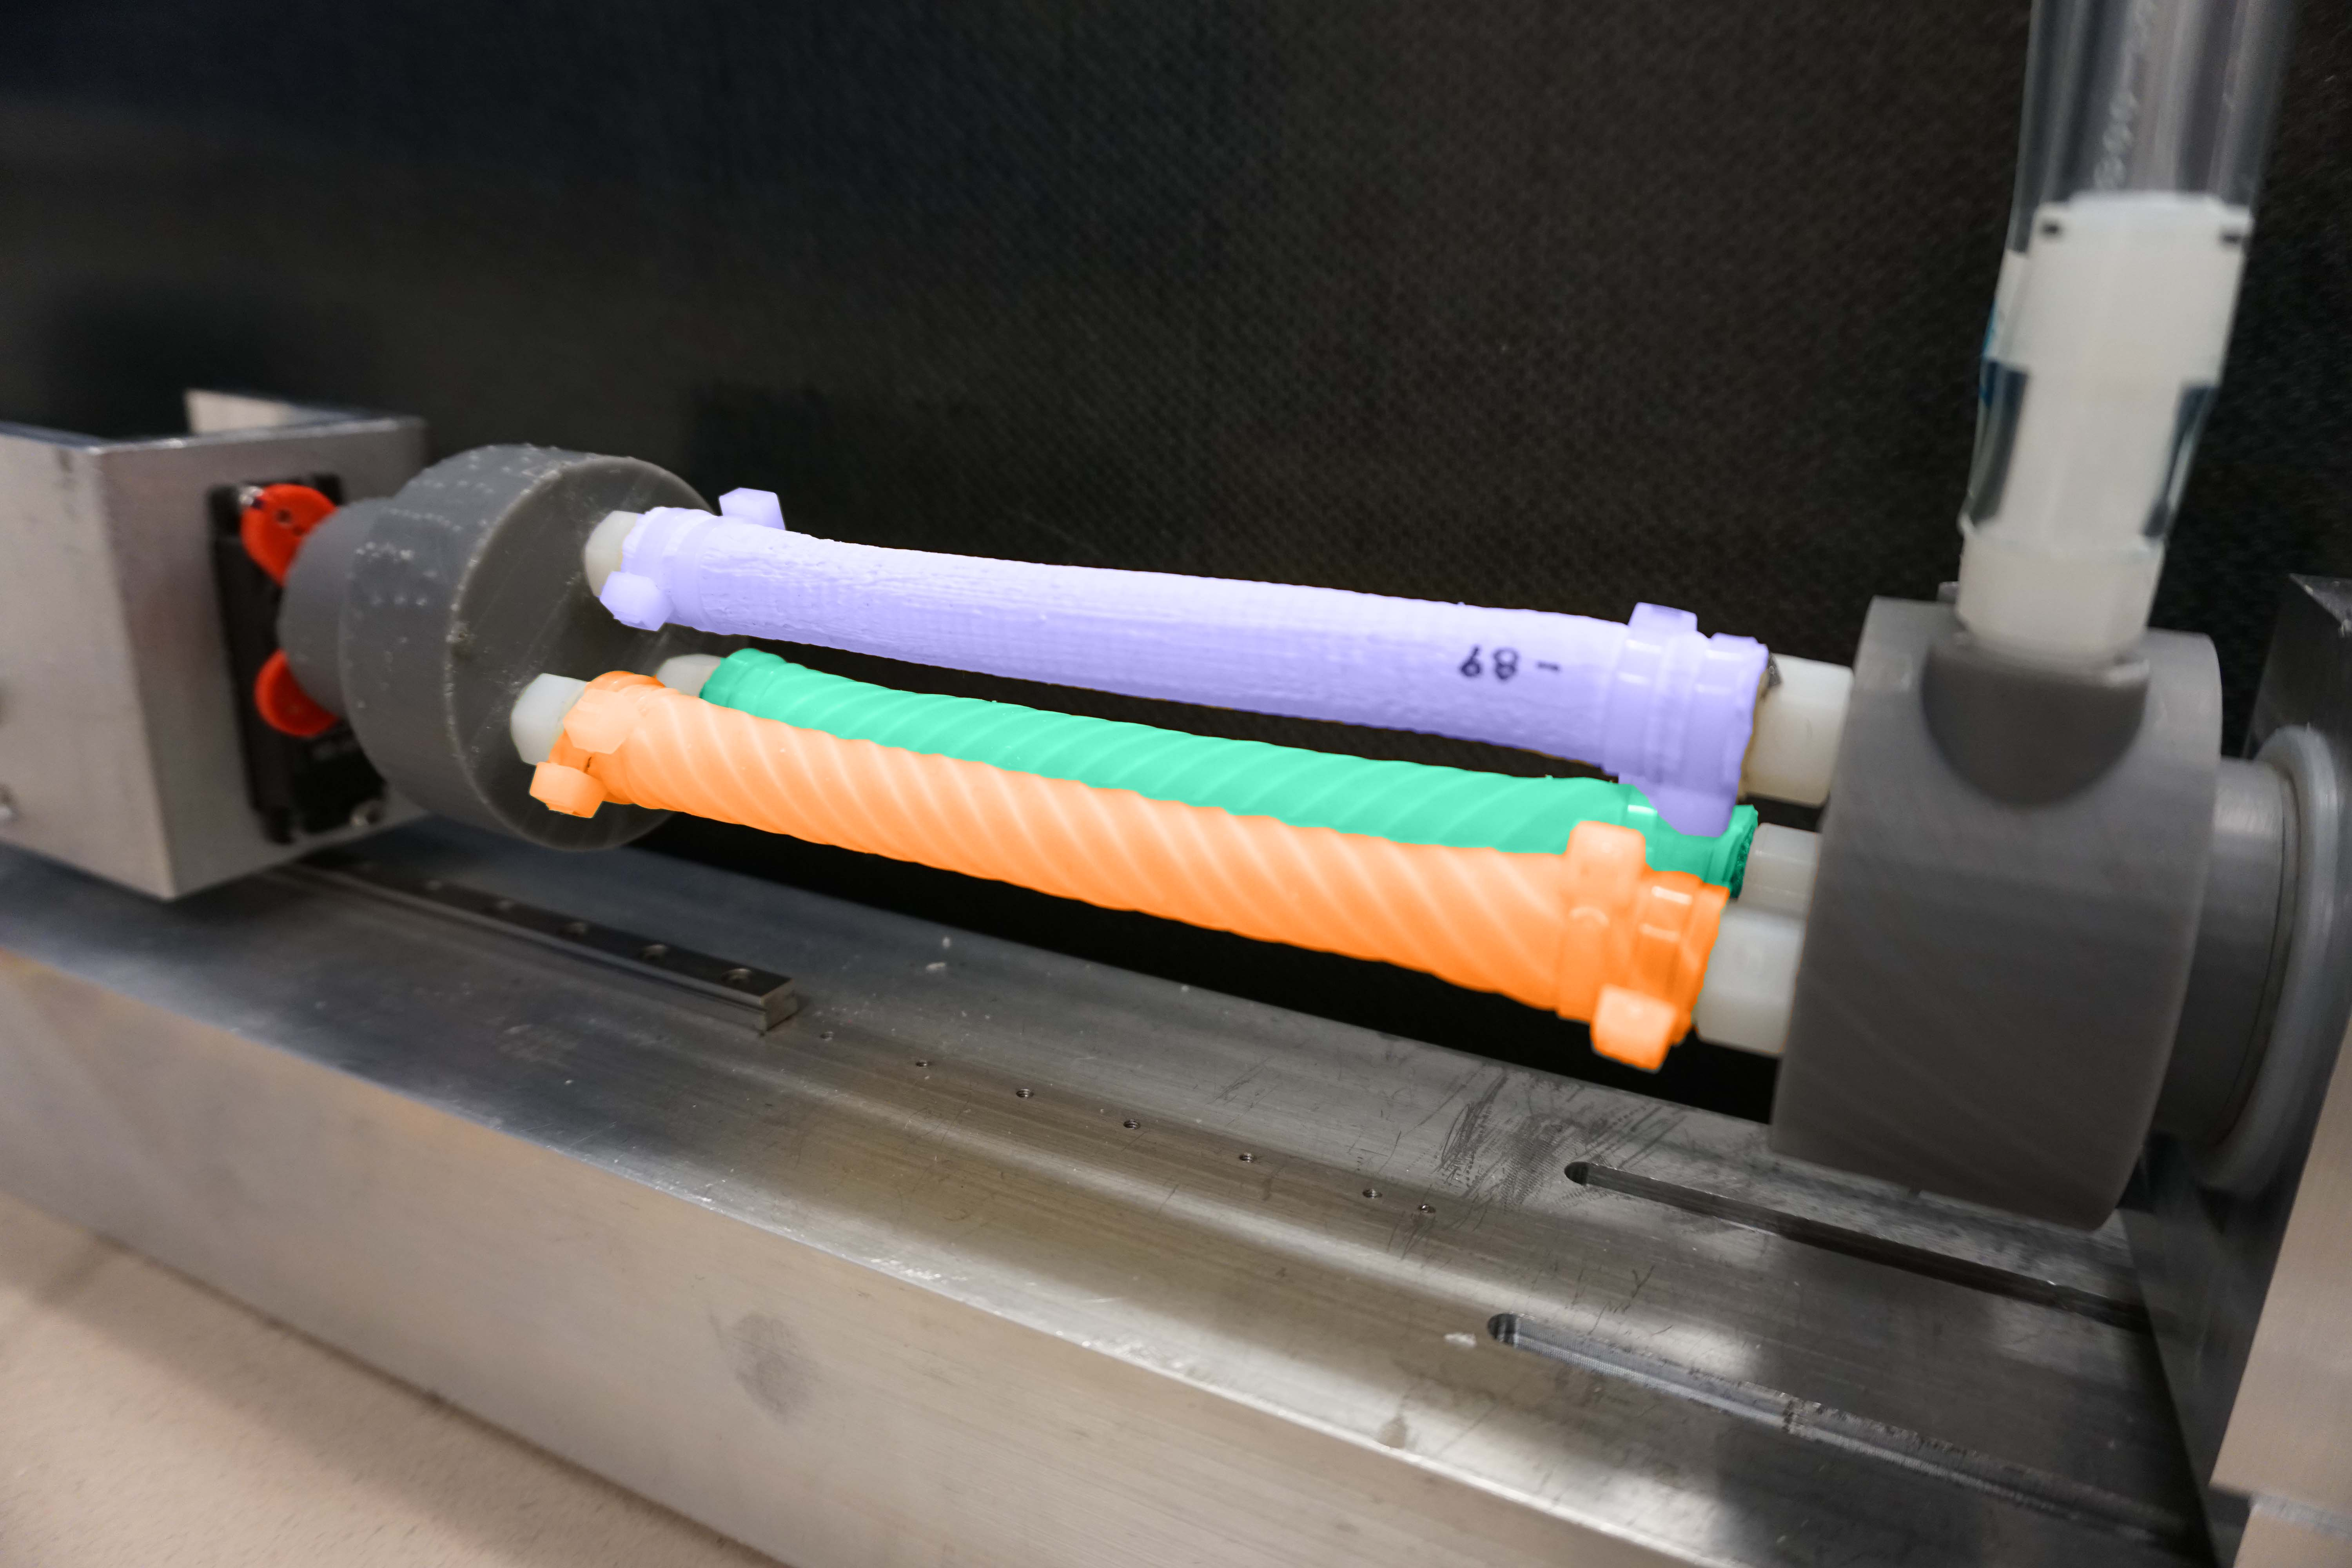
\includegraphics[width=\colWidth]{images/photos/s5w0pic_colored.jpg}}; %\fill[blue] (0,0) circle (2pt);
&
\node[style={anchor=center}] {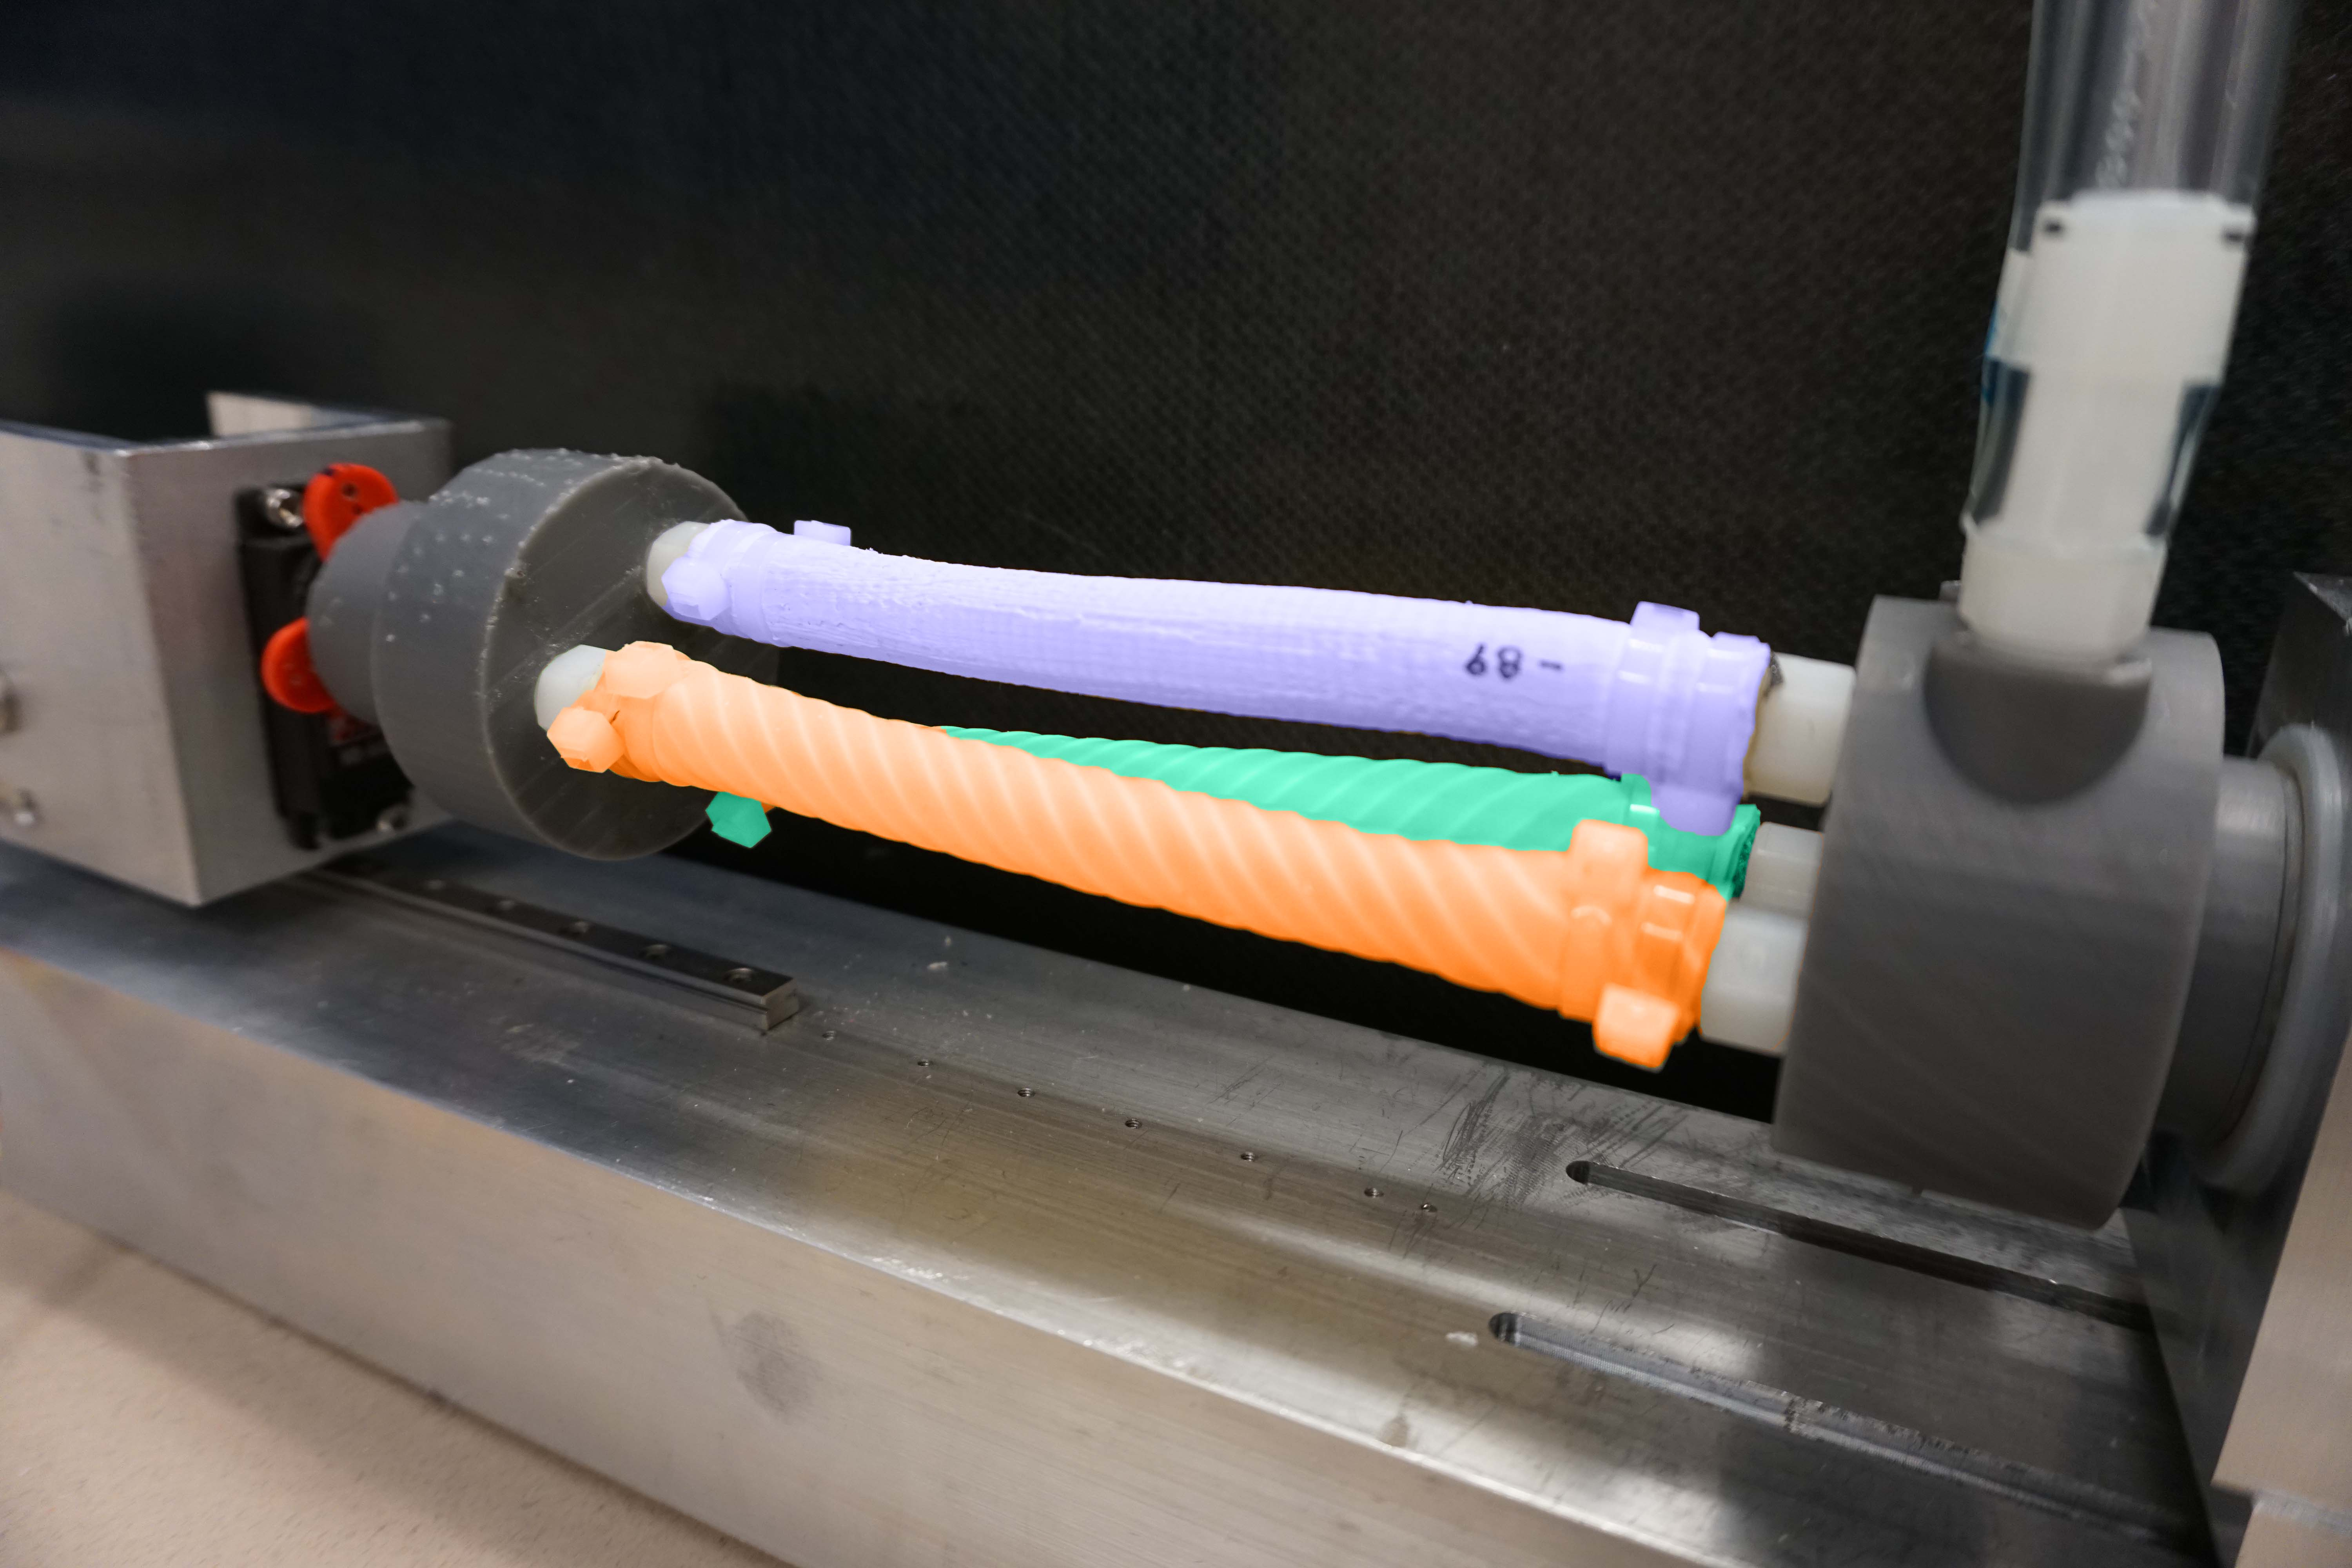
\includegraphics[width=\colWidth]{images/photos/s0w20pic_colored.jpg}}; %\fill[blue] (0,0) circle (2pt);
&
\node[style={anchor=center}] {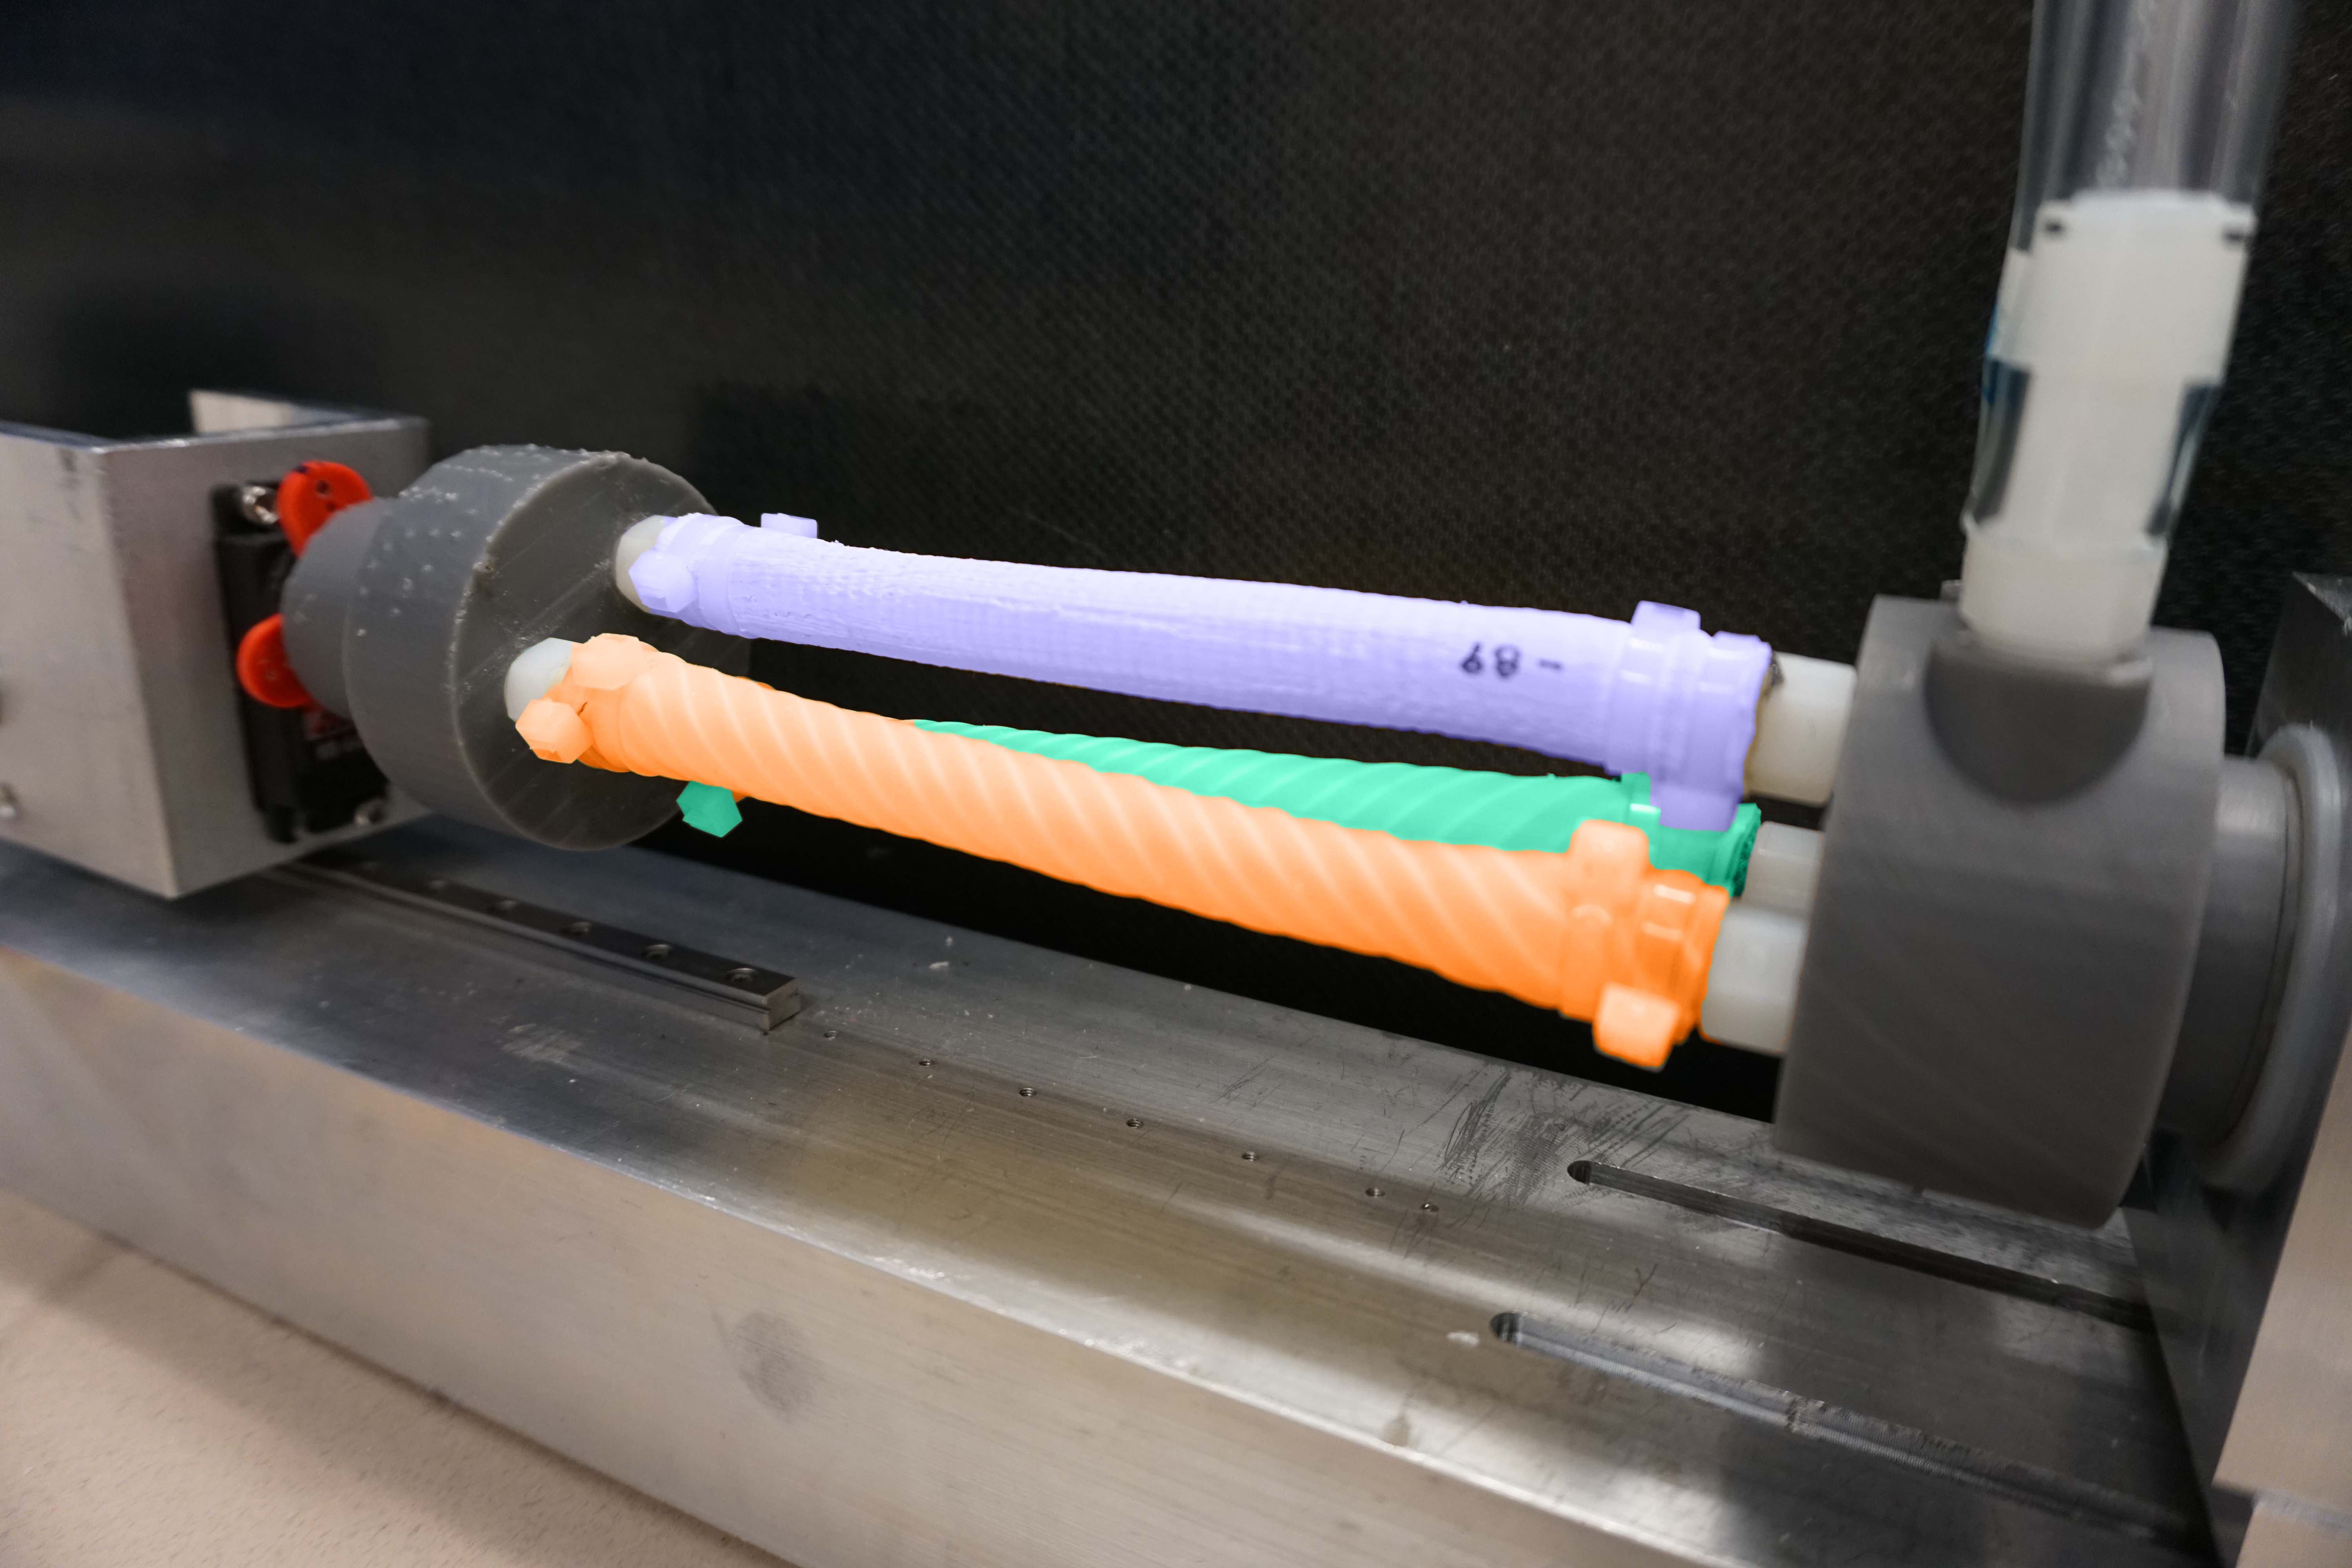
\includegraphics[width=\colWidth]{images/photos/s5w20pic_colored.jpg}}; %\fill[blue] (0,0) circle (2pt);

\\

\node[rotate=90] (ylabel) {Moment, $M^{\hat{z}_e}$ (N-m)};
&
\node[style={anchor=center}] {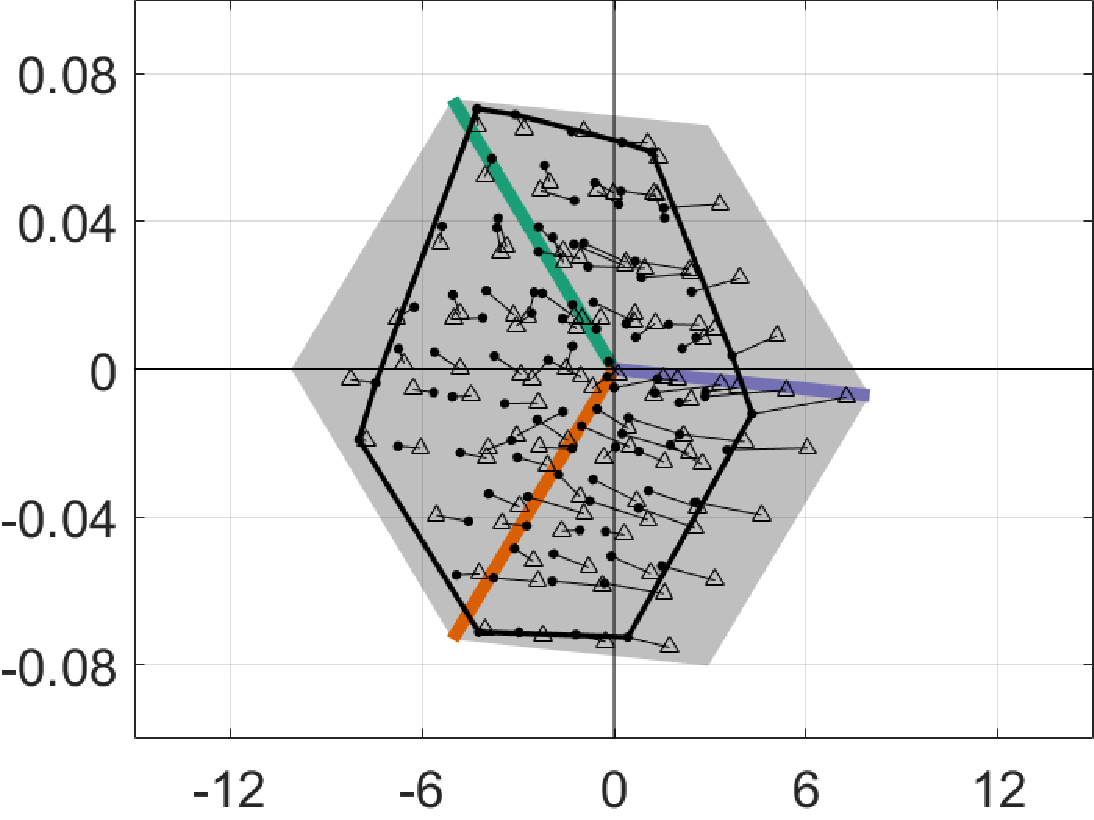
\includegraphics[width=\colWidth]{images/plots/s0w0.pdf}}; %\fill[blue] (0,0) circle (2pt);
&
\node[style={anchor=center}] {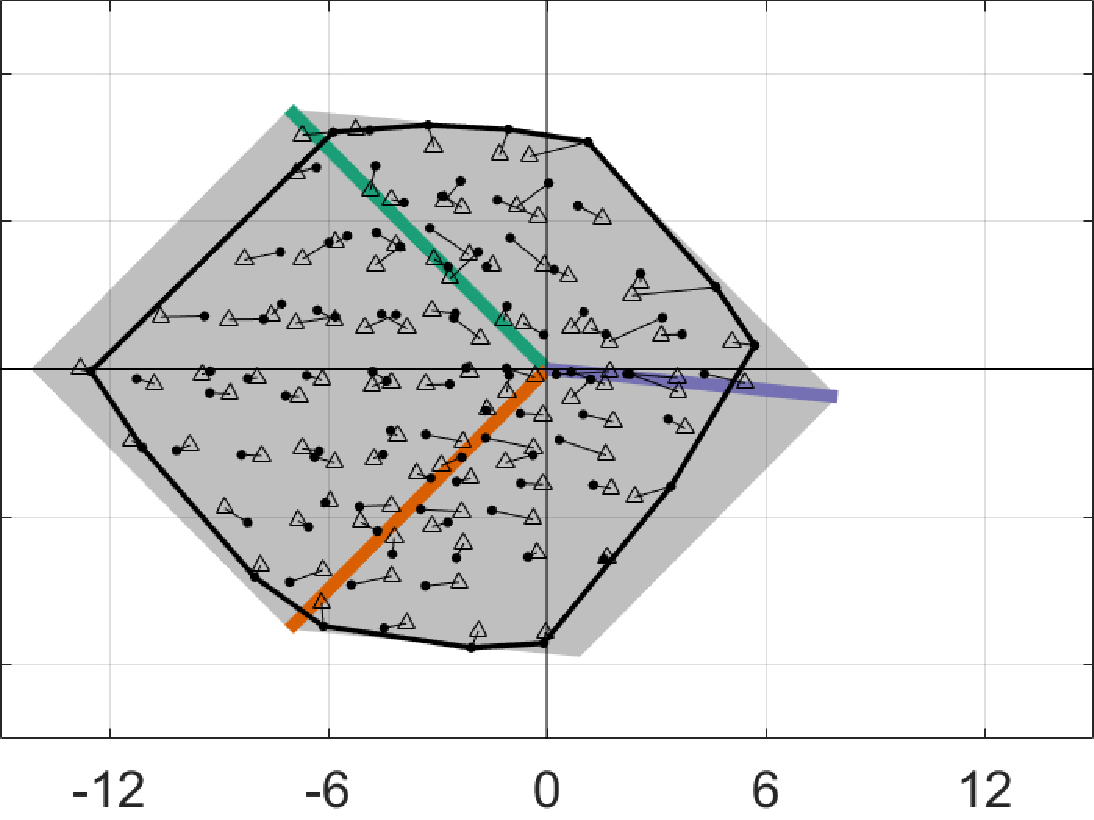
\includegraphics[width=\colWidth]{images/plots/s5w0.pdf}}; %\fill[blue] (0,0) circle (2pt);
&
\node[style={anchor=center}] {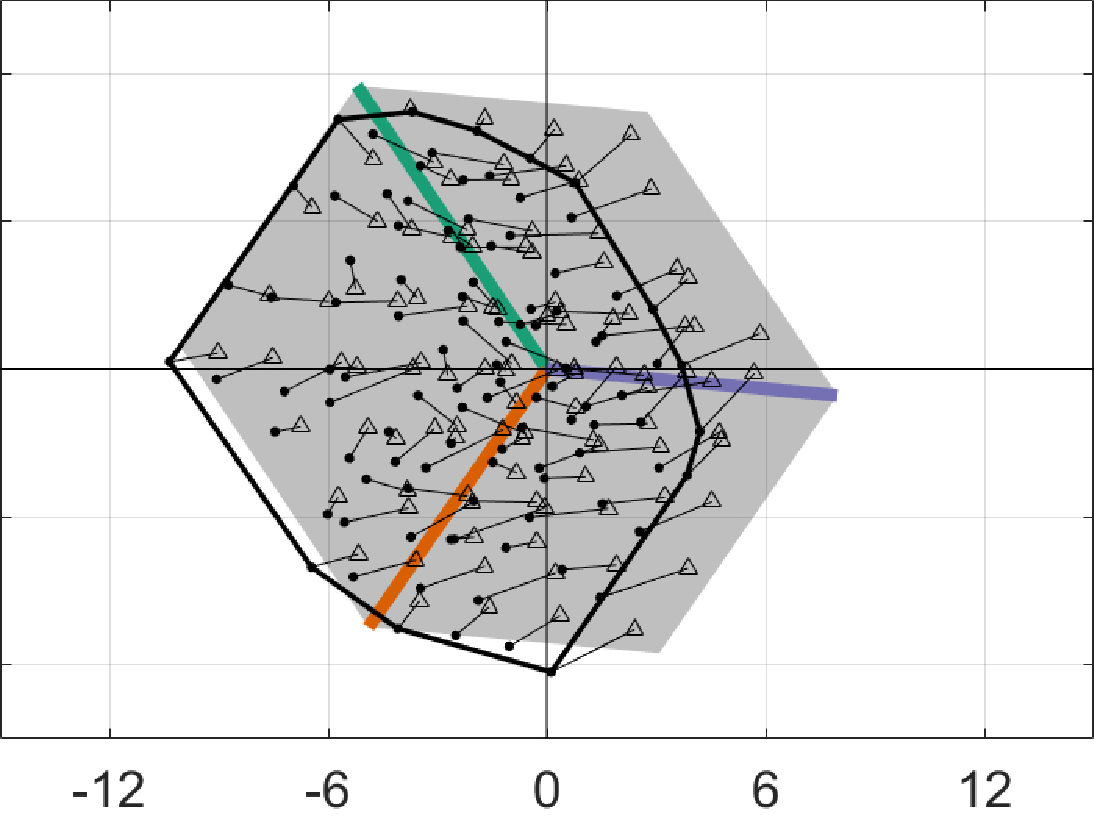
\includegraphics[width=\colWidth]{images/plots/s0w20.pdf}}; %\fill[blue] (0,0) circle (2pt);
&
\node[style={anchor=center}] {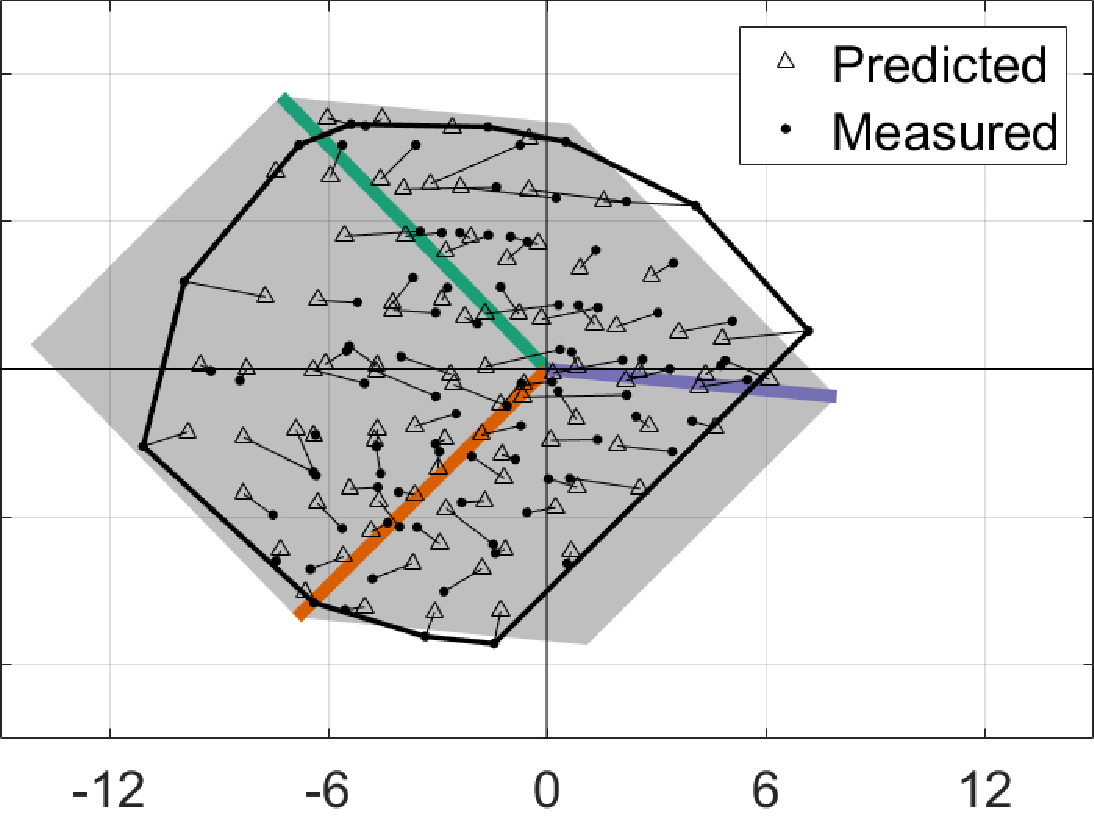
\includegraphics[width=\colWidth]{images/plots/s5w20.pdf}}; %\fill[blue] (0,0) circle (2pt);

\\

& \node (xlabel1) {Force, $F^{\hat{z}_e}$ (N)}; & \node (xlabel2) {Force, $F^{\hat{z}_e}$ (N)}; & \node (xlabel3) {Force, $F^{\hat{z}_e}$ (N)}; & \node (xlabel4) {Force, $F^{\hat{z}_e}$ (N)};

\\
};

\end{tikzpicture}

% \caption{For four different deformed configurations (top row), we compare the predicted and the measured forces for the parallel combination of three FREEs (bottom row). 
% \revcomment{2.6}{Data points and predictions corresponding to the same input pressures are connected by a thin line, and the convex hull of the measured data points is outlined in black.}
% The Trial 1 data is overlaid on top of the theoretical force zonotopes (grey areas) for each of the four configurations.
% Identical colors indicate correspondence between a FREE and its resulting force/torque direction.}
% \label{fig:results}

    \end{minipage}
    
    \begin{minipage}[c]{0.375\linewidth}
        The model predictions matched measured values with root-mean-square error of less than $1.5$ N force and $8 \times 10^-3$ Nm moment.
    \end{minipage}
    \hspace{25pt}
    \begin{minipage}[c]{0.6\linewidth}
    \begin{tikzfigure}
    \centering
    % \caption{Root-mean-square error and maximum error}
    \begin{tabular}{| c | c || c | c | c | c|}
        \hline
        & \rule{0pt}{2ex} \textbf{Disp.} & \multicolumn{2}{c |}{\textbf{RMSE}} & \multicolumn{2}{c |}{\textbf{Max Error}} \\ 
        \cline{2-6}
        & \rule{0pt}{2ex} (mm, $^\circ$) & F (N) & M (Nm) & F (N) & M (Nm) \\
        \hline
        \multirow{4}{*}{\rotatebox[origin=c]{90}{\textbf{Trial 1}}}
        & 0, 0 & 1.13 & $3.8 \times 10^{-3}$ & 2.96 & $7.8 \times 10^{-3}$ \\
        & 5, 0 & 0.74 & $3.2 \times 10^{-3}$ & 2.31 & $7.4 \times 10^{-3}$ \\
        & 0, 20 & 1.47 & $6.3 \times 10^{-3}$ & 2.52 & $15.6 \times 10^{-3}$\\
        & 5, 20 & 1.18 & $4.6 \times 10^{-3}$ & 2.85 & $12.4 \times 10^{-3}$ \\  
        \hline
        % \multirow{4}{*}{\rotatebox[origin=c]{90}{\textbf{Trial 2}}}
        % & 0, 0 & 0.93 & $6.0 \times 10^{-3}$ & 1.90 & $13.3 \times 10^{-3}$ \\
        % & 5, 0 & 1.00 & $7.7 \times 10^{-3}$ & 2.97 & $19.0 \times 10^{-3}$ \\
        % & 0, 20 & 0.77 & $6.9 \times 10^{-3}$ & 2.89 & $15.7 \times 10^{-3}$\\
        % & 5, 20 & 0.95 & $5.3 \times 10^{-3}$ & 2.22 & $13.3 \times 10^{-3}$ \\  
        % \hline
    \end{tabular}
    \label{table:RMSE}
    \end{tikzfigure}
    \end{minipage}
}

% Block 4 - Control
\block{Control: Generate forces in error reducing direction}{
    For position control tasks, a model-based PI controller chooses an input that will generate a force pointing toward the desired end effector location, $\vec{x}_\text{des}$.
    % This controller has been tested in simulation, and will next be implemented on a real system.
    
    \begin{minipage}[c]{0.35\linewidth}
        % A model-based controller solves for the pressures that generate forces 
        The pressure input at the $k^\text{th}$ timestep is generated by solving the linear equation for $\vec{p}_k$:
        
        \vspace{12pt}
        \coloredbox[width=\linewidth, bgcolor=lightgrey, framecolor=lightgrey]{
        \begin{equation*}
            \bar{J}_x^T (\vec{x_k}) \vec{p}_k = \bar{K}_p \vec{e}_k + \bar{K}_I \sum_{i=0}^k \vec{e}_i % + \bar{K}_D (\vec{e}_k - \vec{e}_{k-1}) 
        \end{equation*}
        }
        where $\vec{e}_k = \vec{x}_\text{des} - \vec{x}_k$ is the error at the $k^\text{th}$ time step, and $\bar{K}_p$ and $\bar{K}_i$ are constant gain matrices.
    \end{minipage}
    \hspace{25pt}
    \begin{minipage}[c]{0.6\linewidth}
        \centering
        \begin{tikzpicture}
            \draw (0,0) rectangle (9in, 6in);
        \end{tikzpicture}
    \end{minipage}
}

% Block 5 - References
\block{References/Acknowledgements}{
    [1] Bruder, D., Sedal, A., Vasudevan, R. and Remy, C.D., 2018. Force Generation by Parallel Combinations of Fiber-Reinforced Fluid-Driven Actuators. arXiv preprint arXiv:1805.00124.
    
    \vspace{12pt}
    
    *This material is supported by the Toyota Research Institute, and is based upon work supported by the National Science Foundation Graduate Research Fellowship Program under Grant No. 1256260 DGE.
}

% % Block 6 - Acknowledgements
% \block{Acknowledgements}{
%     *This material is supported by the Toyota Research Institute, and is based upon work supported by the National Science Foundation Graduate Research Fellowship Program under Grant No. 1256260 DGE.
% }


\end{columns}



\end{document}







%% EXTRA STUFF I MIGHT FIND USEFUL %%----------------------------------------------------------------

    % \note[
    %     targetoffsetx=-9cm, 
    %     targetoffsety=-6.5cm, 
    %     width=0.5\linewidth
    %     ]
    %     {e-mail \texttt{sharelatex@sharelatex.com}}
    
% \begin{columns}
%     \column{0.5}
%     \block{A figure}
%     {
%         \begin{tikzfigure}
%             
\includegraphics[width=0.4\textwidth]{images/lion-logo.png}
%         \end{tikzfigure}
%     }
%     \column{0.5}
%     \block{Description of the figure}{\blindtext}
% \end{columns}

% \begin{subcolumns}
%     \subcolumn{0.27} \block{1}{First block.} \block{2}{Second block}
%     \subcolumn{0.4} \block{Sub-columns}{Sample subblocks\\Second subcolumn}
%     \subcolumn{0.33} \block{4}{Fourth} \block{}{Final Subcolumn block}
% \end{subcolumns}

% % Block 4 - Control
% \block{Applications}{
%     \begin{minipage}[c]{0.5\linewidth}
%         \centering
%         
\includegraphics[width=\linewidth]{images/UMlogo.eps}
%     \end{minipage} %
%     \begin{minipage}[c]{0.5\linewidth}
%         \centering
%         
\includegraphics[width=\linewidth]{images/csdl_logo.pdf}
%     \end{minipage}
    
%     \begin{minipage}[c]{\linewidth}
%         \centering
%         \begin{tikzpicture}
%             \node[anchor=center, draw] at (0,0) (poopnode) {Poop};
%         \end{tikzpicture}
%     \end{minipage}
% }